% !TEX encoding = UTF-8 Unicode
% -*- coding: UTF-8; -*-
% vim: set fenc=utf-8

\chapter{Experimentos}%
\label{chap:experimentos}

Esse capítulo apresenta alguns exemplos de experimentos e de simulações computacionais com base em uma aplicação do DfAnalyzer no campo de sedimentação de dinâmica de fluidos computacionais~\cite{silva2016situ}, os quais foram executados a fim de ilustrar a implementação e a utilização do Query Processor --- apresentado no \autoref{chap:rastros-de-proveniencia} ---, assim como os resultados obtidos com as consultas realizadas nos mesmos.

\section{Simulação computacional em sedimentação}

O DfAnalyzer (\textit{c.f.} \autoref{sec:dfanalyzer-uma-instancia-da-arquitetura-armful}) utiliza a \textit{libMesh}, uma biblioteca \textit{open-source} implementada na linguagem C++, desenvolvida para facilitar a simulação de aplicações paralelas de refinamento de malhas e elementos finitos adaptativos~\cite{boncz2008breaking}, em um resolvedor chamado \textit{libMesh-sedimentation}. O propósito dessa aplicação é simular a turbidez e perturbação de correntes de fluidos tipicamente encontradas em processos geológicos. Os sedimentos que são transportados devido à dinâmica e ao movimento dos fluidos computacionais são descritos por um modelo matemático que resulta da equação de incompressibilidade de Navier-Stokes (fluido) combinada com uma equação de transporte dominada por advecção (concentração de sedimentos). A \textit{libMesh-sedimentation} emprega um método de elementos finitos de multi-escala variacional no qual uma abordagem escalonada é utilizada para representar e simular a evolução do tempo nas equações de acoplamento entre o fluido e os sedimentos. 

Nessa aplicação os usuários empregam simulações complexas nas quais grandezas de interesse, tais como resíduos e estimativas de erros, são utilizadas para controlar de forma fina o êxito e a performance da execução~\cite{silva2016situ}. Por exemplo, a convergência ou divergência de valores de determinadas grandezas e atributos, ao longo do tempo, é uma potencial e rica fonte de informação sobre o andamento da simulação computacional. Contudo, em geral, não basta analisar uma única grandeza: frequentemente faz-se necessária a análise dos dados científicos de múltiplos arquivos, gerados em diferentes passos durante a execução do \textit{solver}. Nesse cenário a análise é possibilitada pelo DfAnalyzer o qual, devido a sua arquitetura em componentes herdada da ARMFUL, permite que consultas relacionadas a proveniência e aos dados científicos de múltiplos arquivos e transformações de dados sejam realizadas \textit{on-line}, ainda durante a execução da simulação computacional.

Neste capítulo realizamos várias consultas com um fluxo de dados \(D^{\dagger}\) baseado no \textit{solver} de \textbf{simulação de sedimentação de dinâmica de fluidos computacionais} mencionado nos parágrafos anteriores. Esse fluxo de dados \(D^{\dagger}\) está ilustrado na \autoref{fig:experiments-dataflow}.

\begin{figure}[!htb]
    \centering
    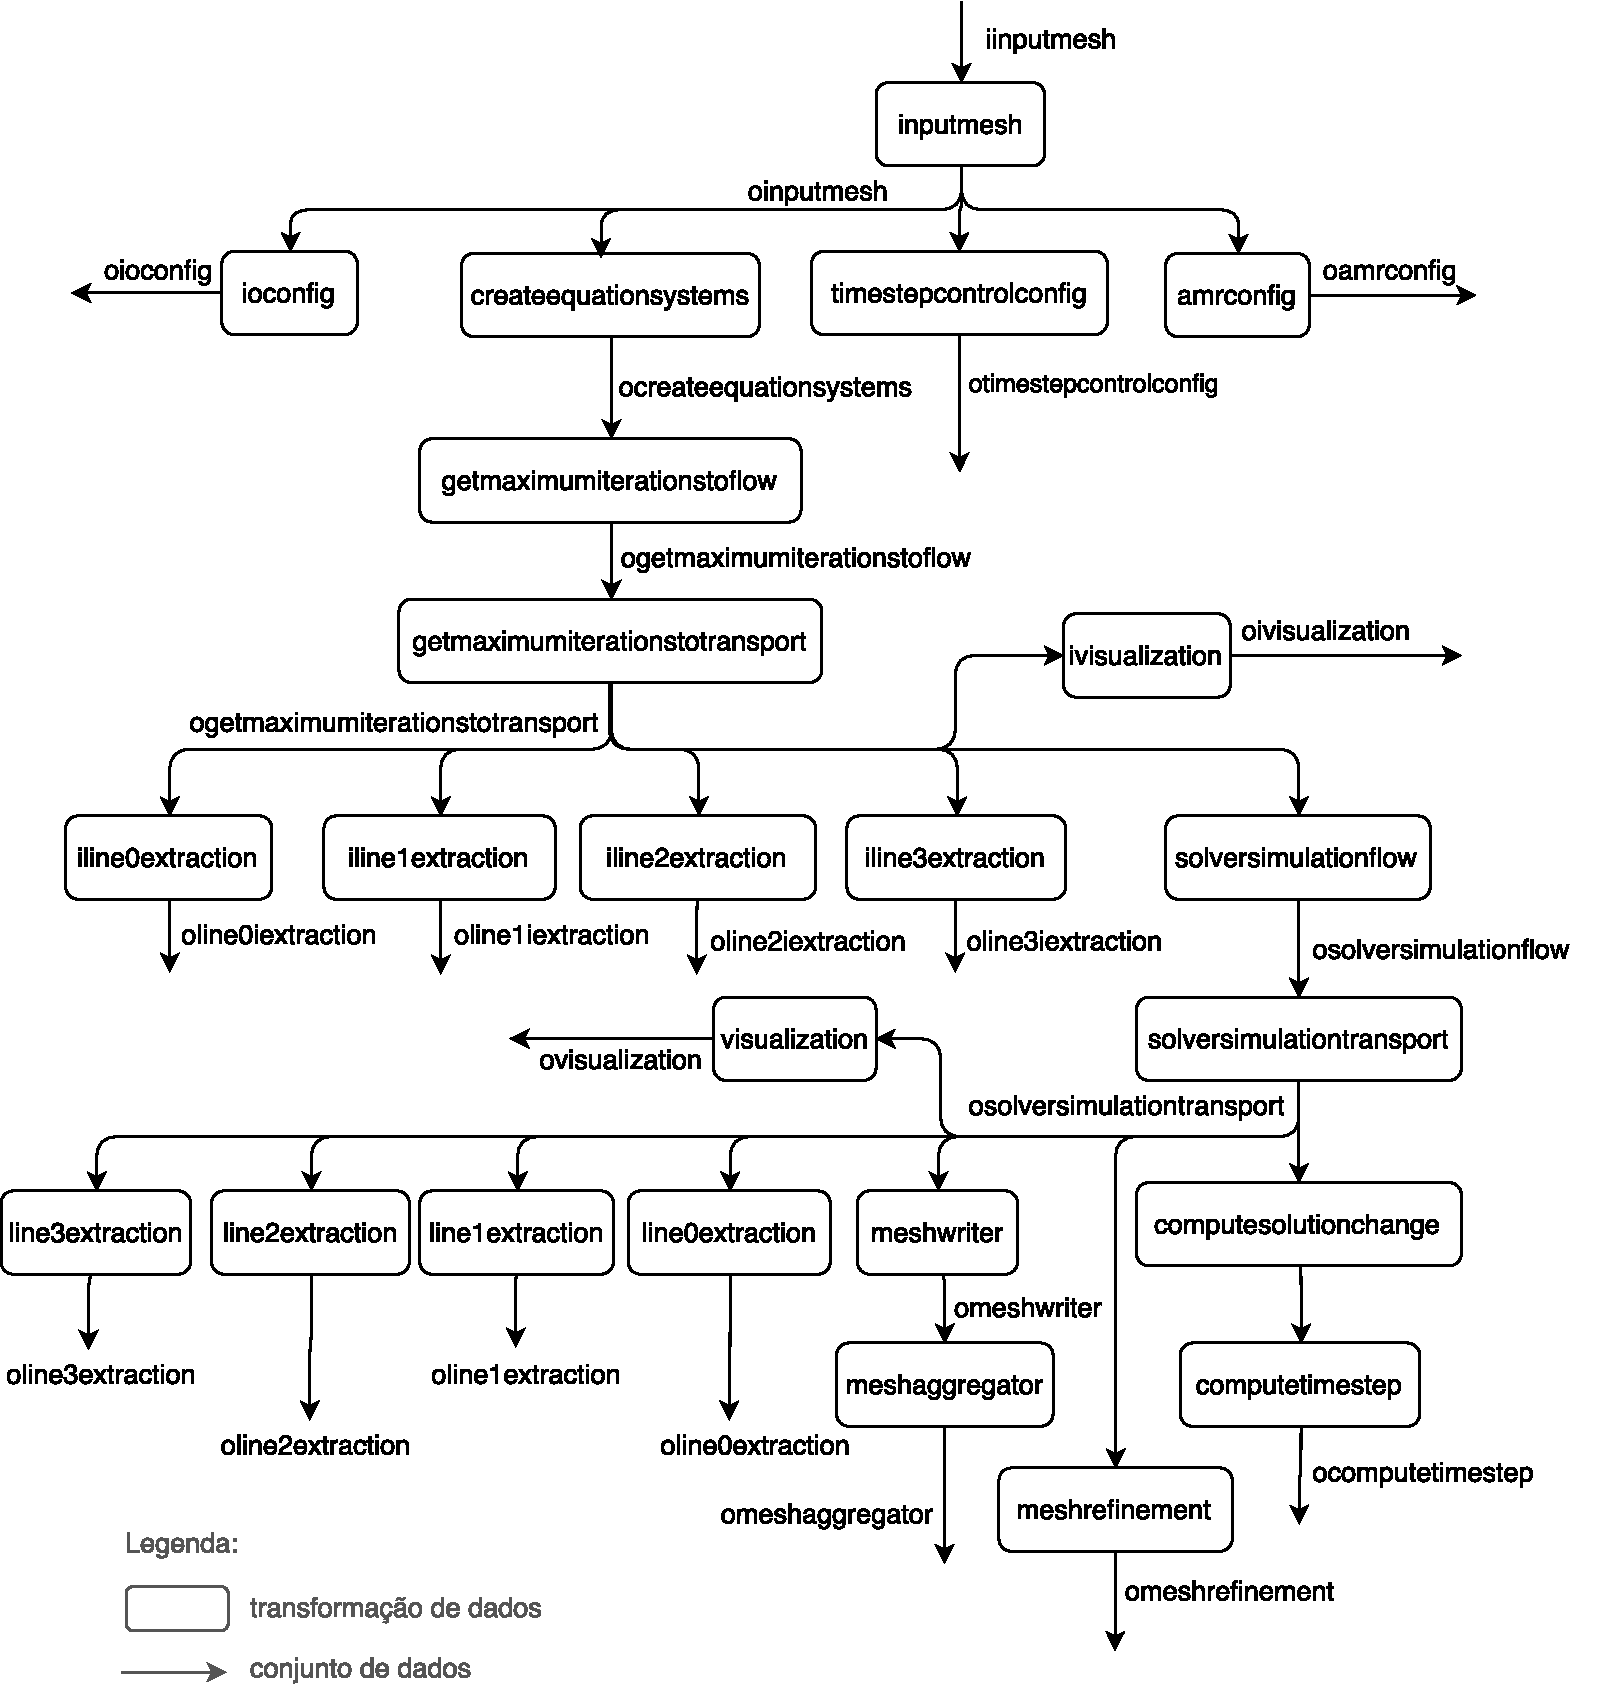
\includegraphics[width=\textwidth]{img/experiments-dataflow}
    \caption[Fluxo de dados $D^{\dagger}$ utilizado nos experimentos]{Fluxo de dados $D^{\dagger}$ utilizado nos experimentos e nas consultas do \autoref{chap:experimentos}.}%
    \label{fig:experiments-dataflow}
\end{figure}

Devido à grande quantidade de conjuntos de dados \(S^{\dagger}\) de \(D^{\dagger}\), não listamos todos os atributos de dados de \(S^{\dagger}\). No entanto, para fins de ilustração, alguns atributos de dados de \(S^{\dagger}\) podem ser visualizados na \autoref{tab:experiments-data-attributes}.

\begin{table}[htb]
    \centering
    \begin{tabular}{c|c|c|c}
\textbf{Conjunto de dados}                  & \textbf{Atributo de dados} & \textbf{Tipo}   & \makecell{\textbf{Exemplo} \\ \textbf{de Valor}}             \\ \hline
\multirow{3}{*}{osolversimulationtransport} & time                       & \makecell{ponto \\ flutuante} & 1e-05                                  \\ \cline{2-4}
                                            & t\_step                    & inteiro         & 0                                      \\ \cline{2-4}
                                            & meshwriter\_task\_id       & inteiro         & 17                                     \\ \hline
\multirow{2}{*}{omeshaggregator}            & xdmf                       & arquivo         & \texttt{\textasciitilde/output\_48.xmf}             \\ \cline{2-4}
                                            & n\_processors              & inteiro         & 480                                    \\ \hline
omeshrefinement                             & first\_step\_refinement    & booleano        & falso                                  \\ \hline
ovisualization                              & png                        & arquivo         & \texttt{\textasciitilde/image\_99.png} \\ \hline
oinputmesh                                  & mesh\_file                 & arquivo         & \texttt{\textasciitilde/necker3d.mesh}               \\ \hline
otimestepcontrolconfig                      & model\_name                & string          & PC11                                  
    \end{tabular}
    \caption[Exemplos de alguns atributos de dados de \(S^{\dagger}\)]{Exemplos de alguns atributos de dados de \(S^{\dagger}\).}%
    \label{tab:experiments-data-attributes}
\end{table}

% \silva{REVIEW: que tipos de arquivos ou dados são coletados na libMesh-sedimentation?. No solver, capturamos dados referentes ao resíduo do solver ao resolver as equações para o fluido e os sedimentos. Para a gerência de arquivos, consideramos os raw data files nos formatos XDMF e HDF5.}

\perrotta{TODO: citar artigo do email}

\section{Experimentos}

As consultas dos experimentos das próximas subseções, relacionadas ao Query Processor, foram executadas em um computador com as seguintes especificações:

\begin{itemize}
	\item Macbook Pro Retina 2015, com o sistema operacional macOS Sierra 10.12.6;
    \item Processador Intel Core i5 2,7~GHz, com 4~CPUs;
    \item 8~GB de memória RAM do tipo DDR3.
\end{itemize}

Quatro consultas foram realizadas, cada uma das quais com diversos parâmetros para a função \texttt{generateSqlQuery} (\textit{c.f.} \autoref{subsec:geracao-da-consulta-em-sql}).

\subsection{Consulta \#1}

A primeira consulta envolve a inspeção de três conjuntos de dados (\texttt{osolversimulationtransport}, \texttt{oline2extraction} e \texttt{omeshwriter}) de \(S^{\dagger}\) e emprega o mapeamento de atributos de dados para rastro de proveniência do tipo físico (\textit{c.f.} \autoref{subsec:rastro-de-proveniencia-do-tipo-fisico}). Apenas duas projeções são de interesse (\texttt{osolversimulation.time} e a média aritmética de \texttt{oline2extraction.d}). A especificação completa da consulta está disponível na \autoref{tab:experiments-1-especificacao}.

\begin{table}[htb]
    \centering
    \begin{tabular}{c|c}
\textbf{Argumento}          & \textbf{Valor} \\ \hline
\texttt{D}                  & $D^{\dagger}$ \\
\texttt{dsOrigins}          & \{\texttt{osolversimulationtransport}\} \\
\texttt{dsDestinations}     & \{\texttt{oline2extraction}, \texttt{omeshwriter}\} \\
\texttt{type}               & physical \\
\texttt{projections}        & \{\texttt{osolversimulationtransport.time}, \texttt{AVG(oline2extraction.d)}\} \\
\texttt{selections}         & \varnothing \\
\texttt{dsIncludes}         & \varnothing \\
\texttt{dsExcludes}         & \varnothing \\
    \end{tabular}
    \caption[Argumentos da função \texttt{generateSqlQuery} para a consulta \#1]{Especificação dos argumentos da função \texttt{generateSqlQuery} para a consulta~\#1.}%
    \label{tab:experiments-1-especificacao}
\end{table}

A consulta \#1 em SQL gerada pelo Query Processor está listada no \autoref{lst:experiments-1-sql}. \textbf{Observação:} uma vez que a função de média aritmética (\texttt{AVG}) é utilizada na projeção, faz-se necessária a utilização da cláusula \texttt{GROUP BY} da linguagem SQL para que a consulta \#1 fique sintaticamente válida e bem definida. Contudo, como o Query Processor não suporta essa cláusula, ela foi adicionada manualmente à consulta gerada pela função \texttt{generateSqlQuery}.

\begin{minipage}[c]{0.95\textwidth}
\begin{lstlisting}[language=sql,label={lst:experiments-1-sql},caption={[Código em SQL gerado na consulta~\#1]Código em SQL gerado na consulta~\#1 (tempo médio: 40,29~ms).}]
SELECT osolversimulationtransport.time, AVG(oline2extraction.d)
FROM osolversimulationtransport, oline2extraction, omeshwriter
WHERE (osolversimulationtransport.line2extraction_task_id = oline2extraction.line2extraction_task_id) 
AND (osolversimulationtransport.meshwriter_task_id = omeshwriter.meshwriter_task_id)
GROUP BY osolversimulationtransport.time;
\end{lstlisting}
\end{minipage}

O resultado da consulta \#1, executada na base de dados de \(D^{\dagger}\) carregada no MonetDB, pode ser visualizado no \autoref{lst:experiments-1-sqlresults}. Uma representação gráfica dos conjuntos de dados de \(S^{\dagger}\) utilizados nessa consulta estão realçados em vermelho na \autoref{fig:experiments-dataflow-1}.

\begin{minipage}[c]{0.95\textwidth}
\begin{lstlisting}[language=sqlresults,label={lst:experiments-1-sqlresults},caption={[Resultados da consulta \#1.]Resultados da consulta \#1 (7 tuplas, tempo médio: 4,346~ms).}]
+--------------------------+--------------------------+
| time                     | L71                      |
+==========================+==========================+
|                1.3398483 |     1.74129306930693e-44 |
|                3.1009347 |  -1.0847045643564339e-44 |
|                5.4124618 |    7.853749801980205e-39 |
|                7.8695609 |  -1.8180726336633645e-33 |
|               10.1307669 |   1.0729463267326738e-27 |
|               12.6055519 |   1.0473414950495052e-24 |
|                       15 |   -8.768540693069305e-22 |
+--------------------------+--------------------------+
\end{lstlisting}
\end{minipage}

\begin{figure}[htb]
    \centering
    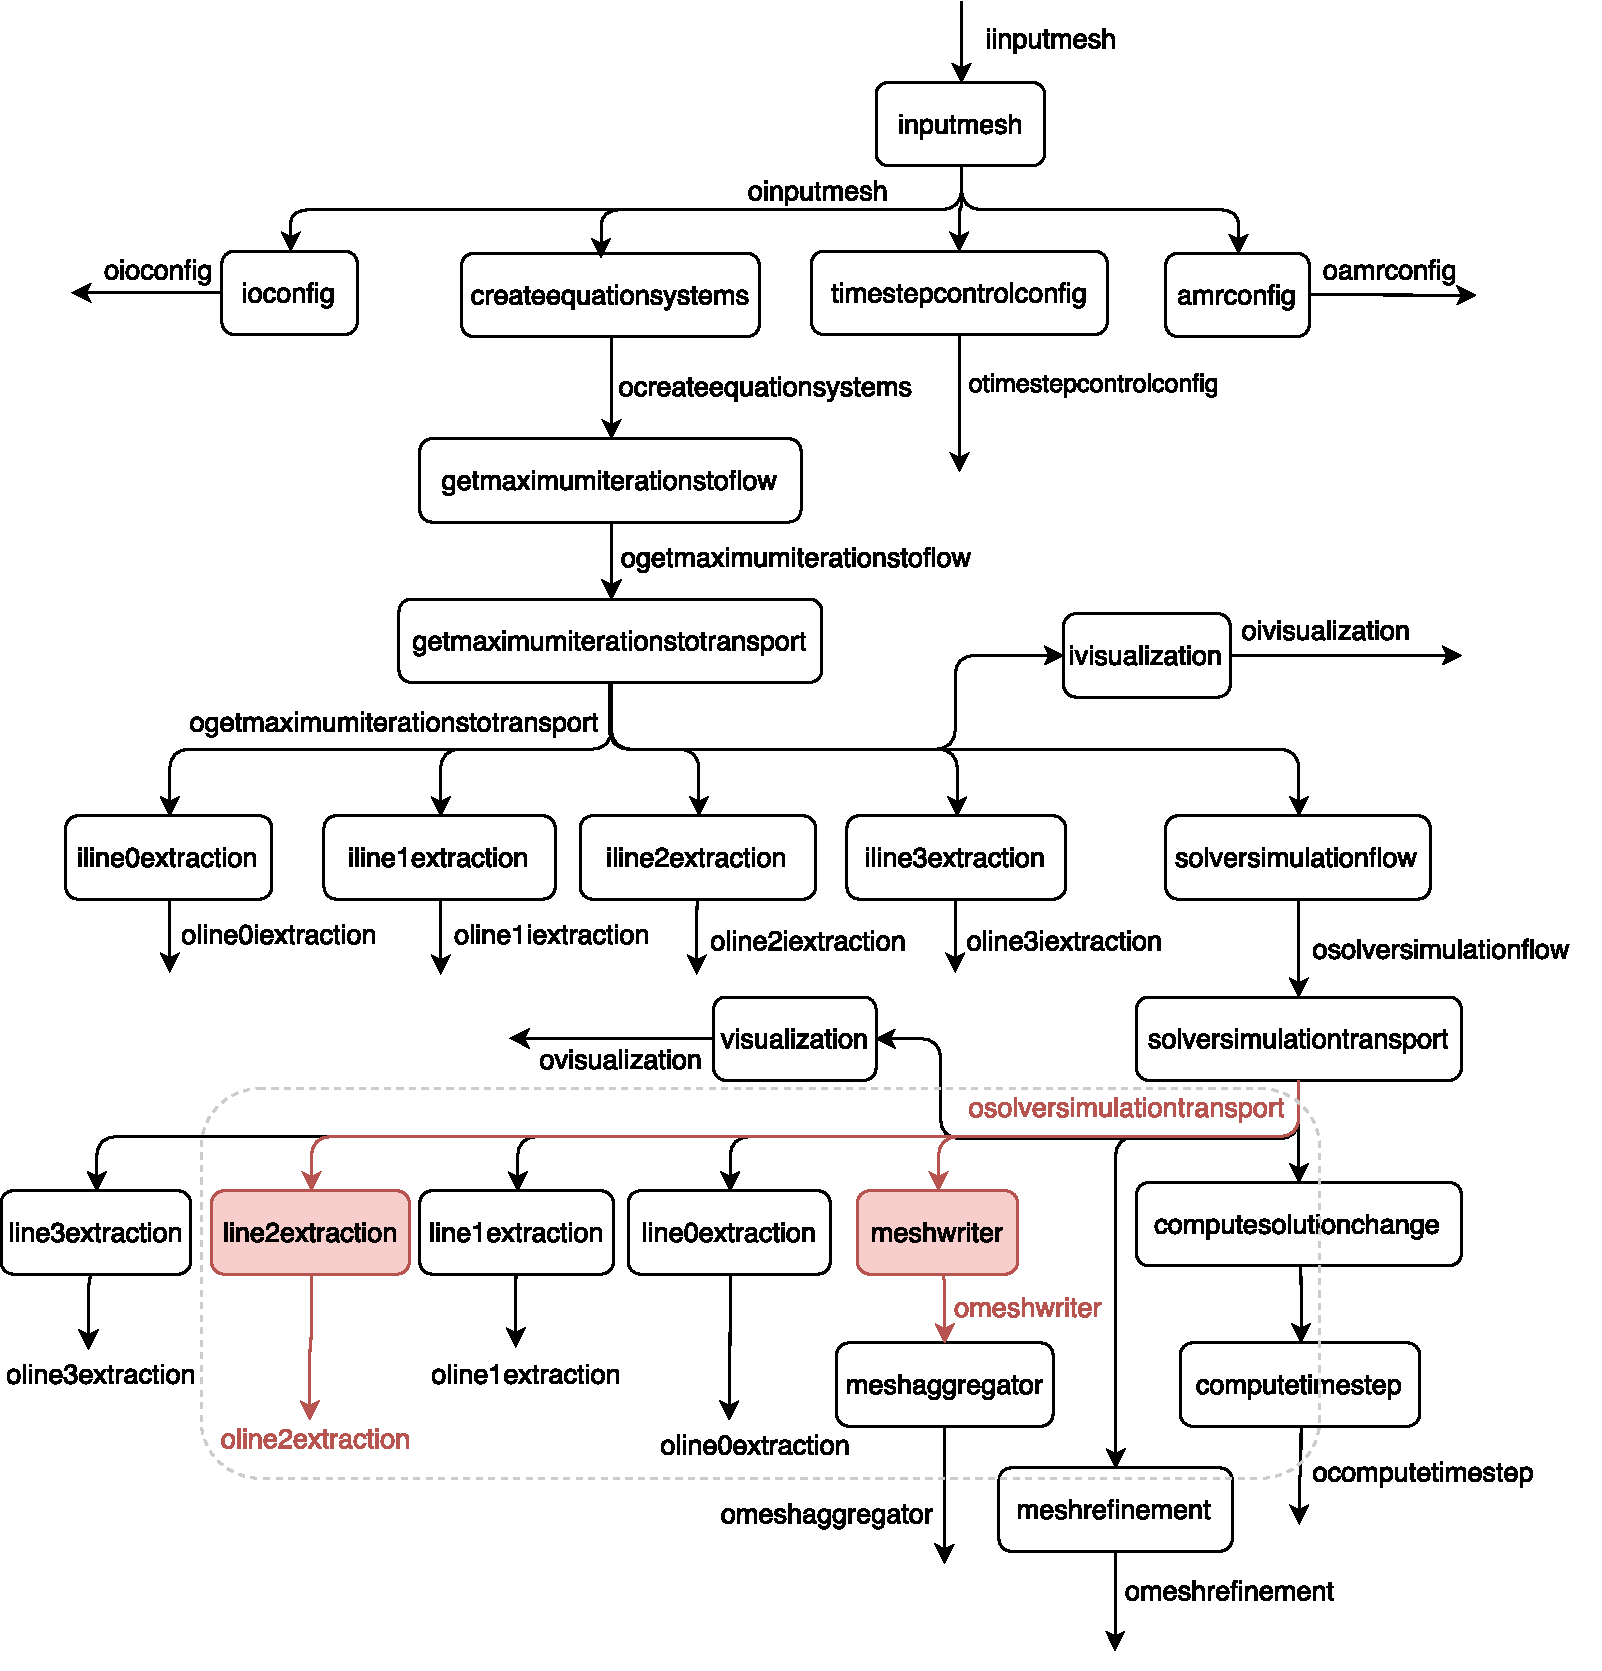
\includegraphics[width=\textwidth]{img/experiments-dataflow-1}
    \caption[Caminho do fluxo de dados \(D^{\dagger}\) rastreado na consulta \#1]{Caminho d fluxo de dados \(D^{\dagger}\) rastreado na consulta \#1.}%
    \label{fig:experiments-dataflow-1}
\end{figure}

\subsection{Consulta \#2}

A segunda consulta ilustra a inspeção de três conjuntos de dados (\texttt{osolversimulationtransport}, \texttt{oline0extraction} e \texttt{omeshwriter}) de \(S^{\dagger}\), empregando o rastro de proveniência do tipo físico. Várias projeções são de interesse para o objetivo de analisar o comportamento do conjunto de dados \texttt{oline0extraction} ao longo do tempo (segundo o atributo de dados \texttt{osolversimulationtransporte.time}). A especificação completa da consulta está disponível na \autoref{tab:experiments-2-especificacao}.

\begin{table}[htb]
    \centering
    \begin{tabular}{c|c}
\textbf{Argumento}          & \textbf{Valor} \\ \hline
\texttt{D}                  & $D^{\dagger}$ \\ \hline
\texttt{dsOrigins}          & \{\texttt{osolversimulationtransport}\} \\ \hline
\texttt{dsDestinations}     & \{\texttt{oline0extraction}, \texttt{omeshwriter}\} \\ \hline
\texttt{type}               & physical \\ \hline
\texttt{projections}        & \makecell{\{\texttt{osolversimulationtransport.time}, \\
                                          \texttt{oline0extraction.points0}, \\ 
                                          \texttt{oline0extraction.points1}, \texttt{oline0extraction.points2}, \\
                                          \texttt{oline0extraction.d}\}} \\ \hline
\texttt{selections}         & \makecell{\{\texttt{osolversimulationtransport.time < 5.5}, \\
                                          \texttt{oline0extraction.d > 0.1}\}} \\ \hline
\texttt{dsIncludes}         & \varnothing \\ \hline
\texttt{dsExcludes}         & \varnothing \\
    \end{tabular}
    \caption[Argumentos da função \texttt{generateSqlQuery} para a consulta \#2]{Especificação dos argumentos da função \texttt{generateSqlQuery} para a consulta~\#2.}%
    \label{tab:experiments-2-especificacao}
\end{table}

A consulta \#2 em SQL gerada pelo Query Processor está listada no \autoref{lst:experiments-2-sql}. \textbf{Observação:} como a cláusula \texttt{LIMIT} não é implementada pelo QP, ela foi adicionada manualmente à consulta após sua geração pela função \texttt{generateSqlQuery}.

\begin{minipage}[c]{0.95\textwidth}
\begin{lstlisting}[language=sql,label={lst:experiments-2-sql},caption={[Código em SQL gerado na consulta~\#2]Código em SQL gerado na consulta~\#2 (tempo médio: 15,45~ms).}]
SELECT osolversimulationtransport.time, oline0extraction.points0, oline0extraction.points1, oline0extraction.points2, oline0extraction.d
FROM osolversimulationtransport, oline0extraction, omeshwriter
WHERE (osolversimulationtransport.time < 5.5) 
AND (oline0extraction.d > 0.1) 
AND (osolversimulationtransport.line0extraction_task_id = oline0extraction.line0extraction_task_id) 
AND (osolversimulationtransport.meshwriter_task_id = omeshwriter.meshwriter_task_id)
LIMIT 10;
\end{lstlisting}
\end{minipage}

O resultado da consulta \#2, executada na base de dados de \(D^{\dagger}\) carregada no MonetDB, pode ser visualizado no \autoref{lst:experiments-2-sqlresults}. Uma representação gráfica dos conjuntos de dados de \(S^{\dagger}\) utilizados nessa consulta estão realçados em vermelho na \autoref{fig:experiments-dataflow-2}.

\begin{lstlisting}[language=sqlresults,label={lst:experiments-2-sqlresults},caption={[Resultados da consulta \#2.]Resultados da consulta \#2 (10 tuplas, tempo médio: 5,92~ms).}]
+--------------+-----------+---------+---------+----------+
| time         | points0   | points1 | points2 | d        |
+==============+===========+=========+=========+==========+
|    5.4124618 |         0 |       1 |       0 |  0.10814 |
|    5.4124618 |      0.18 |       1 |       0 |   0.1082 |
|    5.4124618 |      0.36 |       1 |       0 |  0.10825 |
|    5.4124618 |      0.54 |       1 |       0 |  0.10825 |
|    5.4124618 |      0.72 |       1 |       0 |  0.10825 |
|    5.4124618 |         0 |       1 |       0 |  0.10814 |
|    5.4124618 |      0.18 |       1 |       0 |   0.1082 |
|    5.4124618 |      0.36 |       1 |       0 |  0.10825 |
|    5.4124618 |      0.54 |       1 |       0 |  0.10825 |
|    5.4124618 |      0.72 |       1 |       0 |  0.10825 |
+--------------+-----------+---------+---------+----------+
\end{lstlisting}
% |    5.4124618 |         0 |       1 |       0 |  0.10814 |
% |    5.4124618 |      0.18 |       1 |       0 |   0.1082 |
% |    5.4124618 |      0.36 |       1 |       0 |  0.10825 |
% |    5.4124618 |      0.54 |       1 |       0 |  0.10825 |
% |    5.4124618 |      0.72 |       1 |       0 |  0.10825 |
% |    5.4124618 |         0 |       1 |       0 |  0.10814 |
% |    5.4124618 |      0.18 |       1 |       0 |   0.1082 |
% |    5.4124618 |      0.36 |       1 |       0 |  0.10825 |
% |    5.4124618 |      0.54 |       1 |       0 |  0.10825 |
% |    5.4124618 |      0.72 |       1 |       0 |  0.10825 |

\begin{figure}[htb]
    \centering
    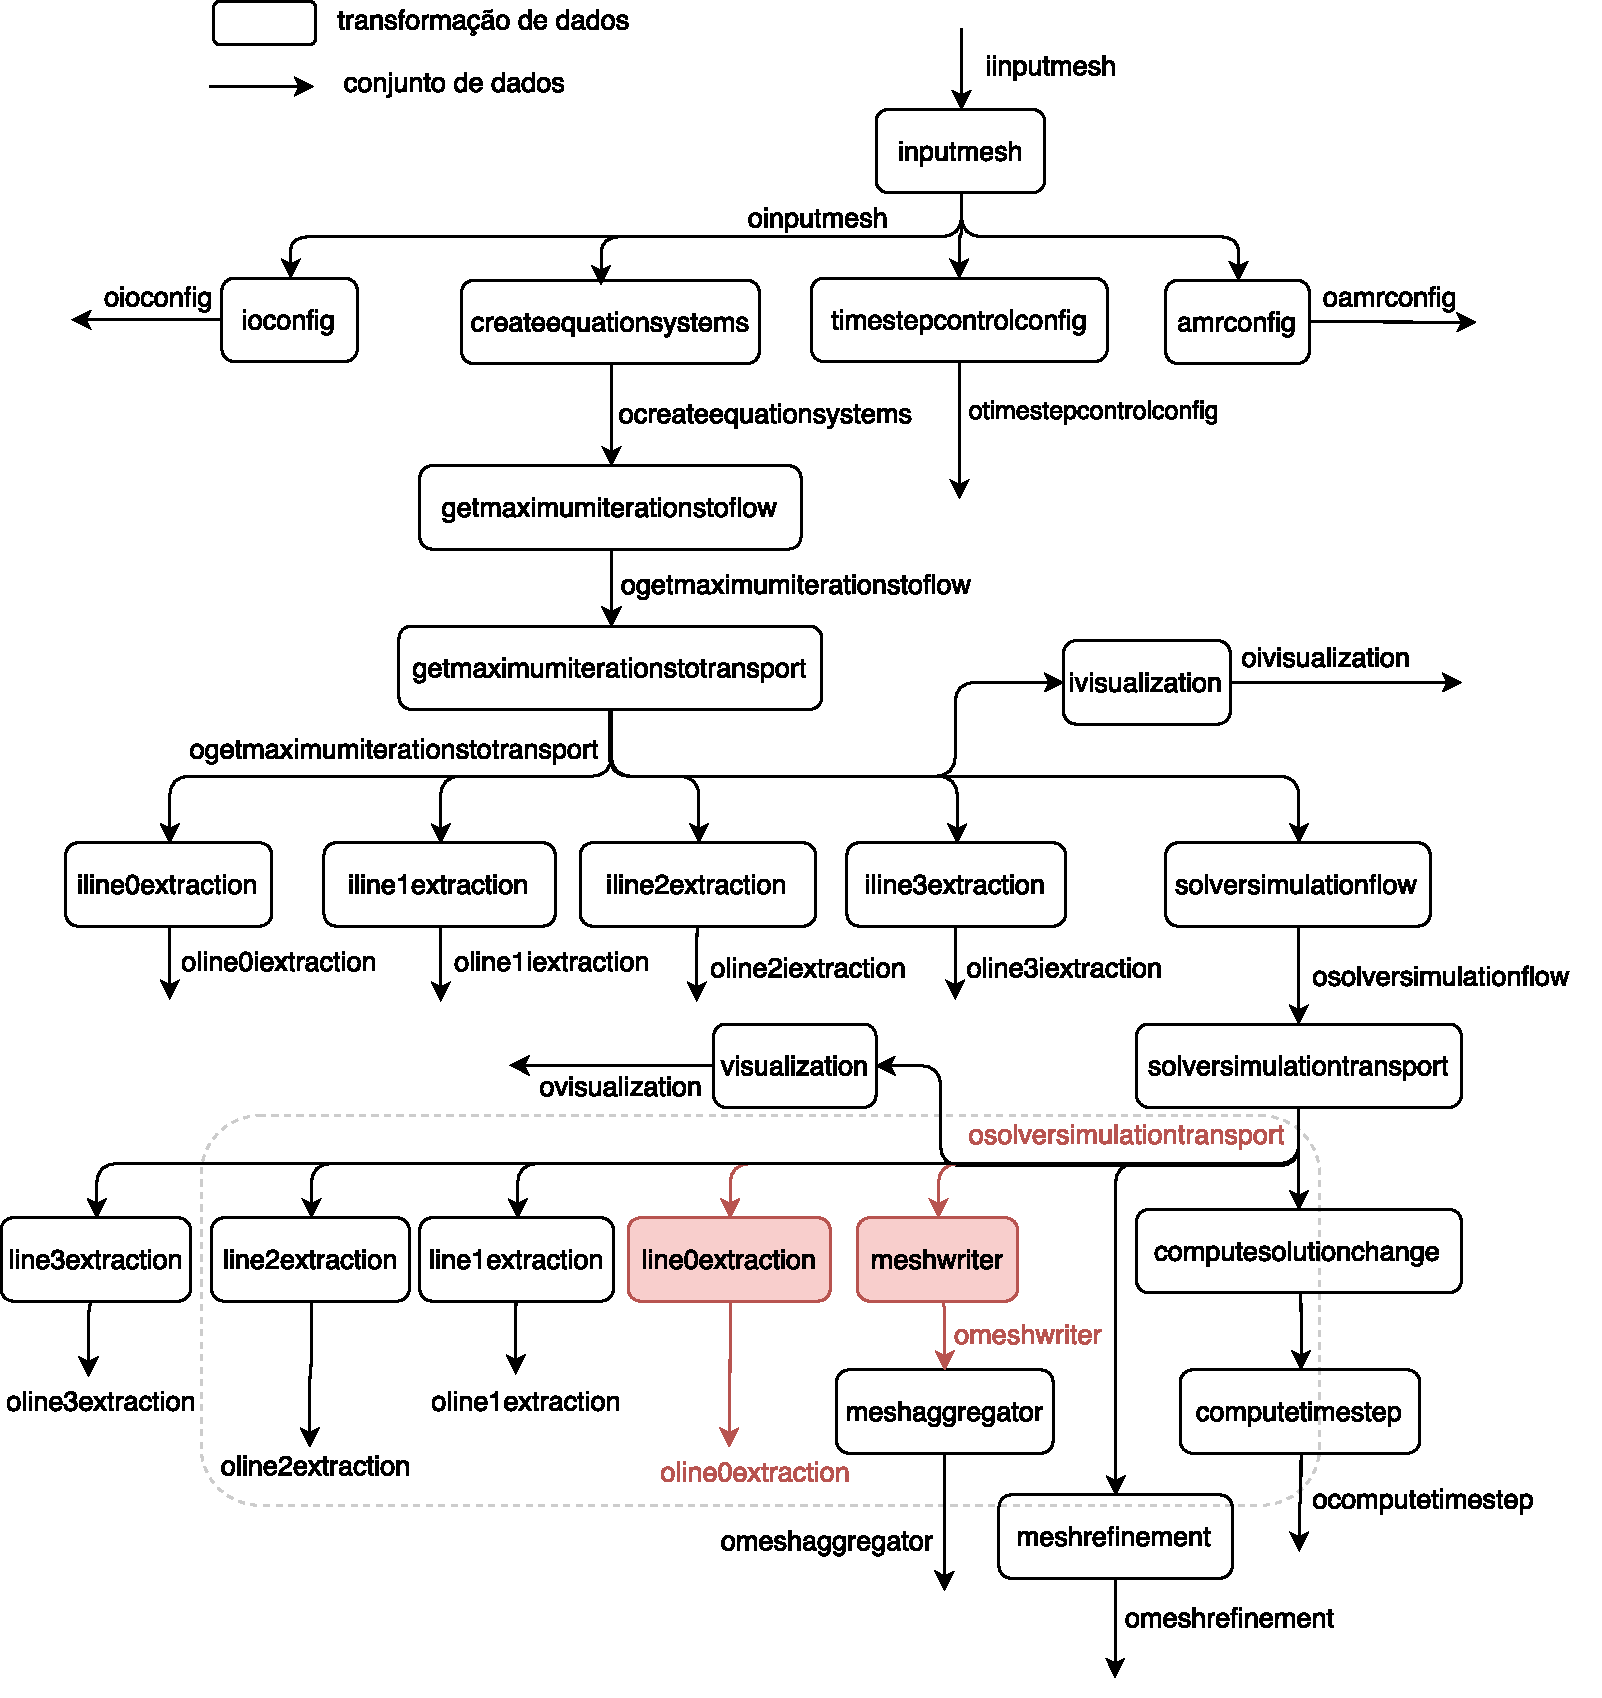
\includegraphics[width=\textwidth]{img/experiments-dataflow-2}
    \caption[Caminho do fluxo de dados \(D^{\dagger}\) rastreado na consulta \#2]{Caminho d fluxo de dados \(D^{\dagger}\) rastreado na consulta \#2.}%
    \label{fig:experiments-dataflow-2}
\end{figure}

\clearpage

\subsection{Consulta \#3}

\perrotta{TODO: consulta \#3}

\subsection{Consulta \#4}

\perrotta{TODO: consulta \#4}

% TODO: mention: Tempo: rodar 4 vezes, tirar a média das 3 últimas